% !TEX root = deckblatt3a.tex

\section{Invertierender Verst\"arker}
\subsection{Simulationsschaltung}
\begin{figure}[H]
  \begin{center}
    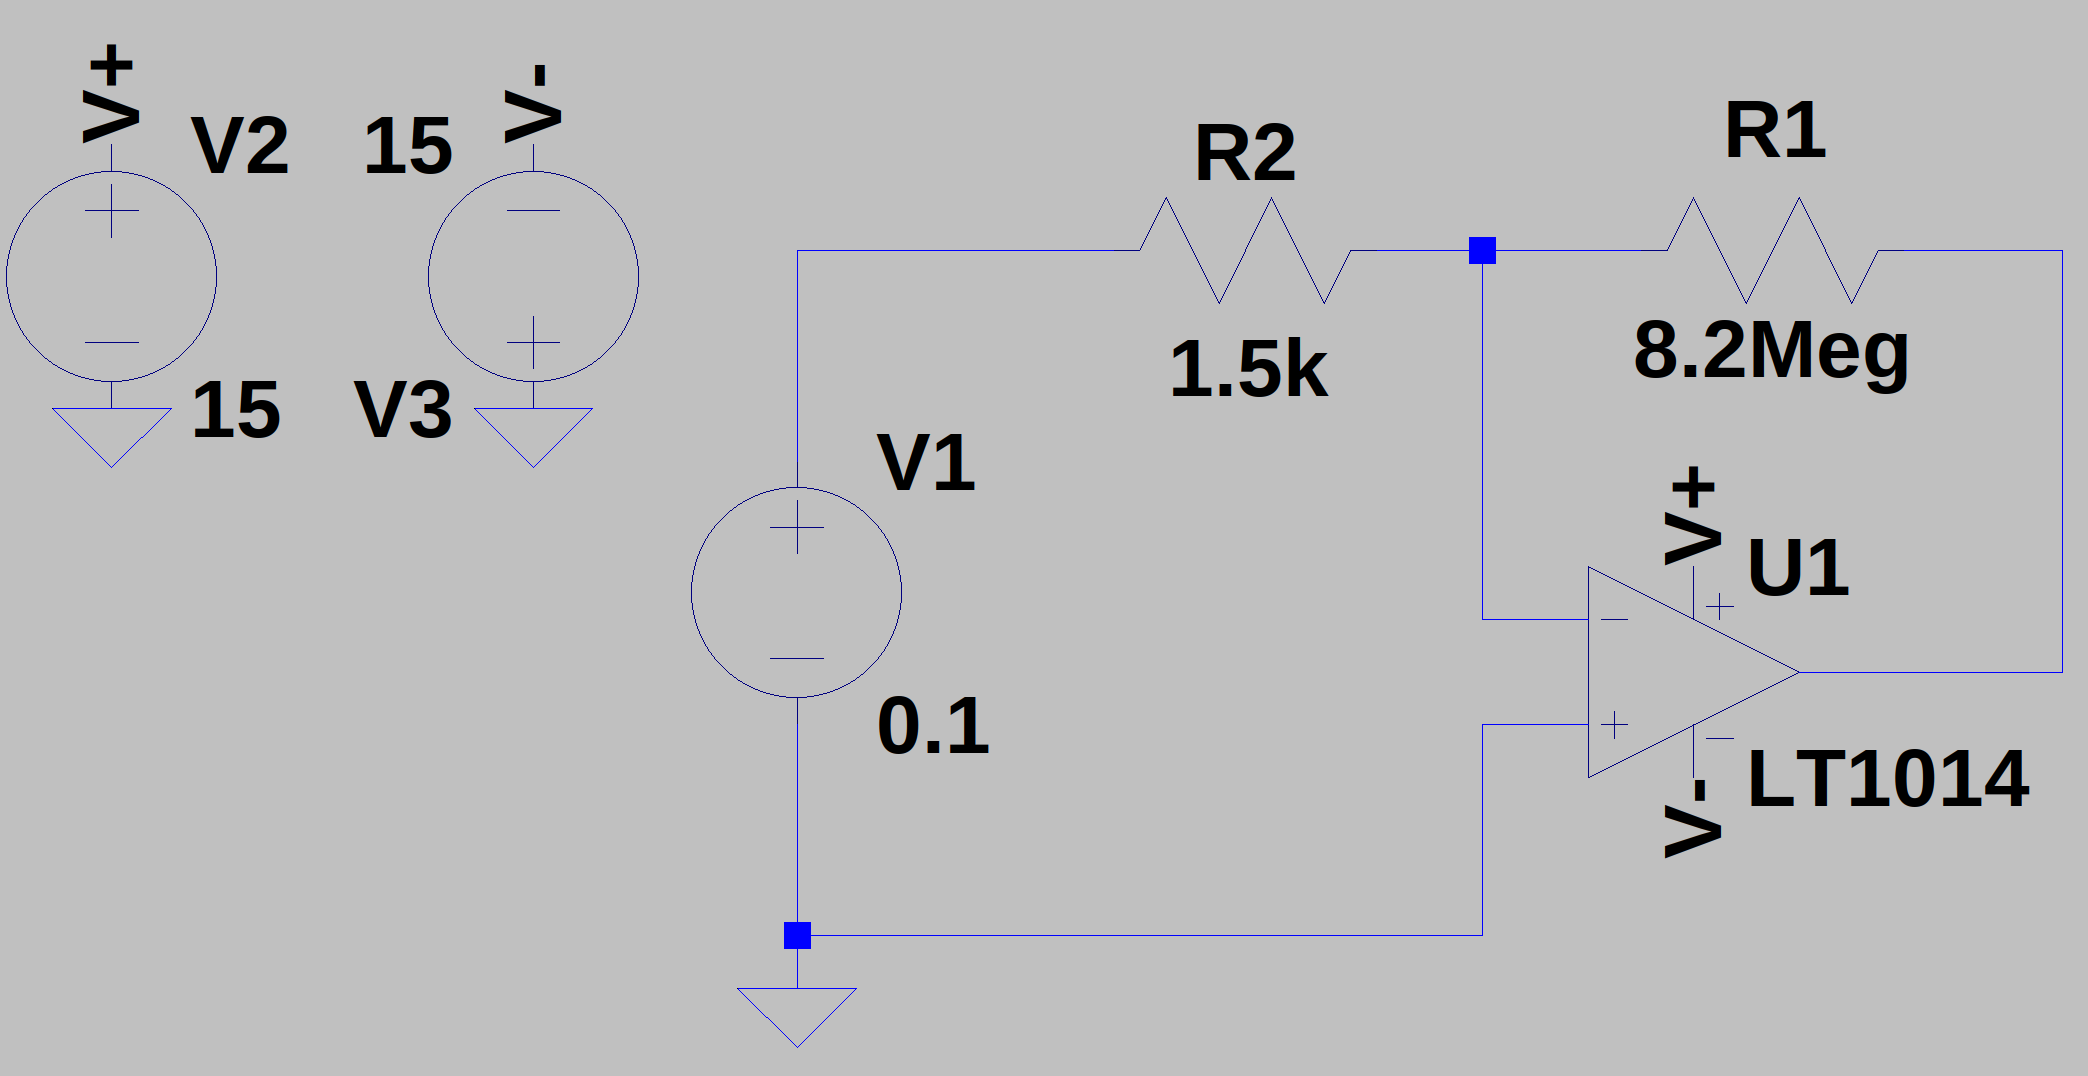
\includegraphics[width=1\textwidth]{./Schaltungen/InvertierenderVerstaerker.png}
    \caption{Simulationsschaltung}
  \end{center}
\end{figure}
\noindent
Da es sich bei dieser Schlatung um einen invertierenden Verst\"arker handelt, wird die Eingangsspannung an den invertierenden Eingang des OPV geschaltet.
Der Ausgang wird ebenfalls auf den invertierenden Eingang gegengekoppelt, um eine brauchbare Verst\"arkung einstellen zu k\"onnen. Ein Idealer OPV ohne Gegenkopplung w\"urde die Differenzspannung zwischen invertierenden und nicht-invertierenden Eingang $\infty$ verst\"arken. Die Verst\"arkung wird mit den beiden Widerst\"anden $R_1$
und $R_2$ eingestellt. Die beiden Spannungsquellen $V_2$ und $V_3$ stellen die symmetrische Versorgungsspannung von $-15V$ bis $+15V$ dar.\\ \\
$\frac{U_e}{U_a}=-\frac{R_1}{R_2} \Rightarrow U_a=-U_e*\frac{R_2}{R_1} \Rightarrow V=-\frac{R_2}{R_1}$ \\ \\
Da sich die Verst\"arkung $V$ laut Angabe zwischen $-40$ und $-60$ befinden soll wurden f\"ur die Widerst\"ande folgende Werte gew\"ahlt: \\ \\
$R_1=82k\Omega$ \\
$R_2=1,5k\Omega$ \\
$V=-\frac{82k \Omega}{1,5k\Omega}=-54,7$

\subsection{Str\"ome und Spannungen}
Am Eingang des invertierenden Verst\"arkers wurde wie in der Simulationsschaltung eine Spannungsquelle mit $100mV$ angeschlossen.

\begin{figure}[H]
  \centering
  \begin{tabular}{c|c||c|c}
    $U_e$ & $100mV$ & & \\ \hline
    $U_a$ & $-5,47V$ & & \\ \hline
    $U_{R_1}$ & $-5,47V$ & $I_{R_2}$ & $-66,68\mu A$  \\ \hline
    $U_{R_2}$ & $100mV$ & $I_{R_1}$ & $-66,68\mu A$  \\ \hline
    $U_{IN-}$ & $786nV$ & $I_{IN-}$ & $-12nA$  \\ \hline
    $U_{IN+}$ & $0V$ & $I_{IN+}$ & $0A$
  \end{tabular}
  \caption{Spannungen und Str\"ome}
\end{figure}
\noindent
Die Ausgangsspannung $U_a$ ergibt sich aus $U_e*V$, in diesem Fall $-5,47V$. Der nicht invertierende Eingang ist auf Masse geschaltet, da ein OPV immer Versucht die Spannung an
beiden Eing\"angen gleich zu halten, befindet sich am invertierenden Eingang die sogenannte "virtuelle Masse". Daraus folgt wiederum, dass an dem Widerstand $R_2$ die $100mV$ der
Eingangs- und an $R_1$ die $-5,47V$ der Ausgangsspannung abfallen. \\
Da der Eingang eines OPV sehr hochohmig ist (ideal: $R_{in}=\infty$) flie\ss{}t auch kein Strom hinein, daraus folgt wiederum dass die Str\"ome durch $R_1$ und $R_2$ gleich
sein m\"ussen.

\subsection{Zeitbereich}
\begin{figure}[H]
  \centering
  \begin{tikzpicture}
    \begin{axis}[width=15cm, height=10cm, xmin=0, xmax=100e-3, xlabel={t}, ylabel={$U[V]$},y tick label style={grid=major}]
      \addplot table[x=time, y=Ue, mark=none] {csv_files/invVer_time1_corr.csv};
      \addplot table[x=time, y=Ua, mark=none] {csv_files/invVer_time1_corr.csv};
    \end{axis}
  \end{tikzpicture}
  \caption{symmetrisches Dreieck, $V_{PP}=0.1V, f=100Hz$}
\end{figure}
\noindent
In dieser Simulation ist ein sch\"ones Verst\"arkerverhalten zu erkennen. Das Eingangsignal, mit einer Amplitude von $V_{PP} = 100mV$, wird mit der zuvor errechneten Verst\"arkung
von $V=-54,7$ verst\"arkt und am Ausgang des OPV ausgegeben.

\begin{figure}[H]
  \centering
  \begin{tikzpicture}
    \begin{axis}[width=15cm, height=10cm, xmin=0, xmax=1e-3, xlabel={t}, ylabel={$U[V]$},y tick label style={grid=major}]
      \addplot table[x=time, y=Ue, mark=none] {csv_files/invVer_time2_corr.csv};
      \addplot table[x=time, y=Ua, mark=none] {csv_files/invVer_time2_corr.csv};
    \end{axis}
  \end{tikzpicture}
  \caption{symmetrisches Dreieck, $V_{PP}=0.1V, f=10kHz$}
\end{figure}
\noindent
Ein realer OPV verh\"alt sich intern \"ahnlich wie ein Tiefpassfilter, je h\"oher die Frequnez desto geringer wird die Verst\"arkung. Dies ist in dieser Simulation sehr gut zu
erkennen, das Ausgangssignal ist im Vergleich zu der vorherigen Messung verschliffen und wird nicht mehr so gut verst\"arkt.


\subsection{Bodediagramme}
\begin{figure}[H]
  \centering
  \begin{tikzpicture}
    \begin{axis}[width=15cm, height=7cm, xmin=1, xmax=100e5, , xmode=log, xlabel={Frequenz [Hz]}, ylabel={Amplitude [dB]},y tick label style={grid=major}]
      \addplot table[x=Frequenz, y=dB,col sep=comma, mark=none] {csv_files/invVer_bode1.csv};
      \node[label={340:{$f_g$}},rectangle,fill=blue,inner sep=3pt] at (axis cs: 39810,7.838) {};
    \end{axis}
  \end{tikzpicture}
  \caption{Amplitudengang, $V=-54,7$}
\end{figure}
\begin{figure}[H]
  \centering
  \begin{tikzpicture}
    \begin{axis}[width=15cm, height=7cm, xmin=1, xmax=100e5, , xmode=log, xlabel={Frequenz [Hz]}, ylabel={Phase [$^\circ$]},y tick label style={grid=major}]
      \addplot table[x=Frequenz, y=Phase,col sep=comma, mark=none] {csv_files/invVer_bode1.csv};
      \node[label={340:{$f_g$}},rectangle,fill=blue,inner sep=3pt] at (axis cs: 39810,112) {};
    \end{axis}
  \end{tikzpicture}
  \caption{Phasengang, $V=-54,7$}
\end{figure}
\noindent
Das zuvor erw\"ahnt Tiefpassverhalten spiegelt sich in dem Bodediagramm wieder. Ab einer Grenzfrequenz von etwa $40kHz$ wird die Verst\"arkung dieser Schaltung weniger und
f\"allt zun\"achst mit $-20dB/Dek$, dies steigt letztlich sogar auf $-40dB/Dek$ an.

\begin{figure}[H]
  \centering
  \begin{tikzpicture}
    \begin{axis}[width=15cm, height=7cm, xmin=1, xmax=100e5, , xmode=log, xlabel={Frequenz [Hz]}, ylabel={Amplitude [dB]},y tick label style={grid=major}]
      \addplot table[x=Frequenz, y=dB,col sep=comma, mark=none] {csv_files/invVer_bode2.csv};
      \node[label={340:{$f_g$}},rectangle,fill=blue,inner sep=3pt] at (axis cs: 199526,-8.194) {};
    \end{axis}
  \end{tikzpicture}
  \caption{Amplitudengang, , $V=-5,47$}
\end{figure}
\begin{figure}[H]
  \centering
  \begin{tikzpicture}
    \begin{axis}[width=15cm, height=7cm, xmin=1, xmax=100e5, , xmode=log, xlabel={Frequenz [Hz]}, ylabel={Phase [$^\circ$]},y tick label style={grid=major}]
      \addplot table[x=Frequenz, y=Phase,col sep=comma, mark=none] {csv_files/invVer_bode2.csv};
      \node[label={340:{$f_g$}},rectangle,fill=blue,inner sep=3pt] at (axis cs: 199526,116) {};
    \end{axis}
  \end{tikzpicture}
  \caption{Phasengang, $V=-5,47$}
\end{figure}
\noindent
Bei diesem Bodediagramm wurde die Verst\"arkung von $V=-54,7$ auf $V=-5,47$ verringert, dies erfolgte durch eine Veringerung von $R_1$ auf $8,2k\Omega$. Durch das
\"Andern der Schaltungseigenschaften verschiebt sich die Grenzfrequenz des OPV nach hinten. Anstatt bereits bei $40kHz$ beginnt die D\"ampfung bei dieser Schaltung erst ungef\"ahr
eine Dekade sp\"ater bei etwa $200kHz$.
